% -*- LaTeX -*-
% -*- coding: utf-8 -*-
%
% michael a.g. aïvázis
% california institute of technology
% (c) 1998-2012 all rights reserved
%

\lecture{Survival skills}{20120109}

% --------------------------------------
% overview
\begin{frame}[fragile]
%
  \frametitle{Sources of complexity}
%
  \begin{itemize}
%
  \item problem size 
    \begin{itemize}
      \item cpu time, amount of memory, cpu count
    \end{itemize}
%
  \item project size
    \begin{itemize}
    \item asset complexity: lines of code, entry points, files
    \item dependencies: number of modules, third party libraries
    \item run-time complexity: number of object types and instances
    \end{itemize}
%
  \item project longevity
    \begin{itemize}
    \item duty cycle, life cycle
    \item cost/benefit of reuse
    \item managing change: people, software, hardware, technology
    \end{itemize}
%
  \item locality of needed resources
    \begin{itemize}
    \item computation and persistence: where, how, when, who
    \end{itemize}
%
  \item usability
    \begin{itemize}
    \item learning curve, ease of access, interfaces, security, etc.
    \end{itemize}
%
  \end{itemize}
%
\end{frame}

% --------------------------------------
% risk mitigation
\begin{frame}[fragile]
%
  \frametitle{Risk mitigation}
%
  \begin{itemize}
%
  \item verification and validation
    \begin{itemize}
    \item invariants, consistency checks, code introspection
    \item benchmark problems
    \item reality checks
    \end{itemize}
%
  \item key software practices
    \begin{itemize}
    \item source control: e.g. cvs; svn; git, hg, bzr
    \item uniform build procedure: platforms, compilers, dependencies, but also build types
    \item testing: unit, component, application; mutation, regression; {\em automate}
    \item tracking of bugs and feature requests: gnats, bugzilla, trac
    \item documentation: doxygen, epydoc; wiki
    \item code reviews
    \end{itemize}
%
  \item project coherence
    \begin{itemize}
    \item design methodology
    \item flexible software architecture
    \item coding and documentation standards
    \item regular meetings
    \end{itemize}
%
  \end{itemize}
%
\end{frame}

% --------------------------------------
% remote access
\begin{frame}[fragile]
%
  \frametitle{Remote access to computational resources}
%
  \begin{itemize}
%
  \item \ssh, the {\em secure shell}:
    \begin{itemize}
    \item currently the most flexible and secure method
    \item authentication, strong data encryption
    \item interactive sessions, remote shell services, data transfer, command execution
    \end{itemize}
%
  \item authentication requires a {\em private} and a {\em public} key
    \begin{itemize}
    \item the private key is protected by a {\em passphrase}; must be long enough to be
      difficult to guess, but memorable because it is not recoverable
    \item you only need one private key, and it only needs to be installed on machines whose
      keyboard you actually touch
    \item you install your public key on every machine to which you require access
      \begin{itemize}
        \item on unix machines: in \url{~/.ssh/authorized_keys}
      \end{itemize}
    \item keys are created using \sshkeygen; on windows there is \putty
    \end{itemize}
%
  \item most installations support {\tt\small ssh-agent}
    \begin{itemize}
    \item a wrapper around your interactive session that asks you for your passphrase, loads
      your private key in memory, and negotiates authentication with \ssh\ servers
      automatically
    \end{itemize}
%
  \end{itemize}
%
\end{frame}

% --------------------------------------
% key generation with putty
\begin{frame}[fragile]
%
  \frametitle{Key generation with {\tt PuTTY}}
%
  \begin{itemize}
  \item the \putty\ screen before and after a key has been generated
  \end{itemize}

\vspace{.25in}
%
  \begin{minipage}{.45\linewidth}
    \begin{figure}
      \centering
      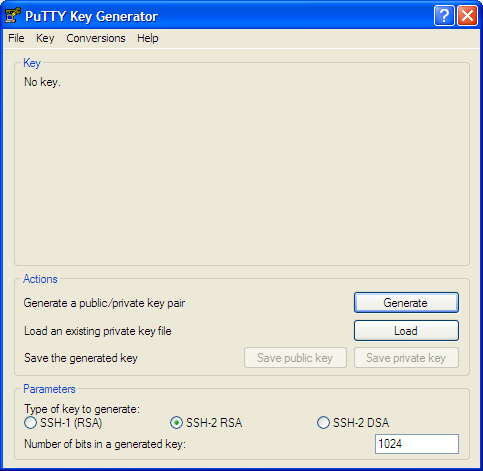
\includegraphics[scale=0.25]{figures/putty-initial.png}
    \end{figure}
  \end{minipage}
%
  \hfill
%
  \begin{minipage}{.45\linewidth}
    \begin{figure}
      \centering
      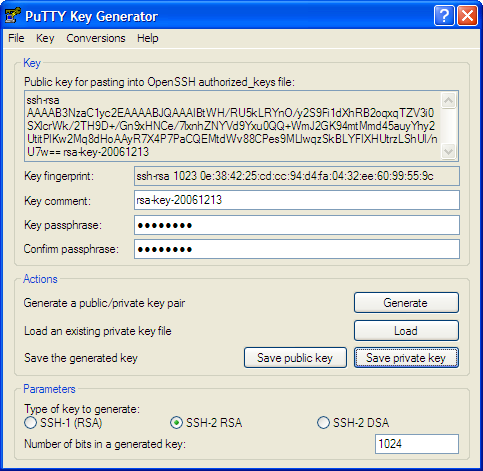
\includegraphics[scale=0.25]{figures/putty-key.png}
    \end{figure}
  \end{minipage}
%
\end{frame}

% --------------------------------------
% bazaar
\begin{frame}[fragile]
%
  \frametitle{Bazaar -- setup}
%
  \begin{itemize}
%
  \item we are going to use \bzr, a source control system, for both homework and final project
    submissions
%
  \item installation instructions, documentation and tutorials available from
    \href{http://bazaar.canonical.com}
%
  \item bazaar keeps track of authors in its revision history, so it's a good idea to give it
    your name and an email address
%
    \begin{shell}{}
#> bzr whoami "Michael Aivazis <aivazis@caltech.edu>"
    \end{shell}
%
    \item you should verify that it worked by asking
%
      \begin{shell}{}
#> bzr whoami
Michael Aivazis <aivazis@caltech.edu>
      \end{shell}
%
    \item the discussion here is specialized to the class repository, but the ideas generalize
      easily
%
  \end{itemize}
%
\end{frame}

% --------------------------------------
% bazaar initialization
\begin{frame}[fragile]
%
  \frametitle{Bazaar -- initialization}
%
  \begin{itemize}
%
  \item first, decide where you would like to place the folder with the homework repository,
    open a terminal window, and change your working directory to
%
  \item create a new repository
%
    \begin{shell}{}
#> bzr init acm114
Created a standalone tree (format: 2a)
    \end{shell}
%
  \item \bzr\ will create the new folder for you and initialize it; change your working
    directory to the new folder
    \begin{shell}{}
#> cd acm114
    \end{shell}
%
  \item you can ask \bzr\ for details about the current repository
    \begin{shell}{}
#> bzr info
Standalone tree (format: 2a)
Location:
  branch root: .
    \end{shell}
%
  \item \bzr\ commands are {\em repository global}: they apply to the entire repository, unless
    explicitly restricted to a particular file or folder
%
  \end{itemize}
%
\end{frame}

% --------------------------------------
% bazaar pull
\begin{frame}[fragile]
%
  \frametitle{Getting information from the class server}
%
  \begin{itemize}
%
  \item \bzr\ is a {\em distributed} source control system: each repository has a copy of the
    entire change history, and can evolve independently
%
  \item you are responsible for sharing information among repositories by invoking the
    repository synchronization commands {\em explicitly} and providing the location of the
    remote repository
%
  \item populate your new {\tt\small acm114} repository by {\em pulling} from the class server
    \begin{shell}{}
#> bzr pull --remember bzr+ssh://acm114@acm114.caltech.edu
+N  assigment-1/                                                                                   
+N  assigment-1/20120120.pdf
+N  assigment-1/20120120.tex
+N  assigment-1/setup.tex
All changes applied successfully.                                                                  
Now on revision 1.
    \end{shell}
%
  \item {\tt\small --remember} asks bzr to use the class repository as the default: afterwards,
    you can just {\tt\small bzr pull} without mentioning the source
  \item {\tt\small bzr+ssh} is the connection scheme that employs \ssh\ for authentication
  \item \url{acm114@acm114.caltech.edu} is the address of your homework repository on the class
    server
  \end{itemize}
%
\end{frame}

% --------------------------------------
% work cycle 
\begin{frame}[fragile]
%
  \frametitle{Working in the repository}
%
  \begin{itemize}
%
  \item one of the problems in the first assignment asks you to write a routine that computes
    the first few terms of some series in a language of your choice; let's assume that you
    picked {\tt\small python}, and you created a file {\tt\small dilog.py}
    \begin{shell}{}
#> cd assignment-1
#> vi dilog.py
    \end{shell}
%
  \item you can inform \bzr\ that you would like to place {\tt\small dilog.py} under source
    control
    \begin{shell}{}
#> bzr add dilog.py
adding assigment-1/dilog.py
    \end{shell}
%
  \item let's check what \bzr\ knows about the repository
    \begin{shell}{}
#> bzr status
added:
  assigment-1/dilog.py
    \end{shell}
%
  \end{itemize}
%
\end{frame}

% --------------------------------------
% committing and submitting
\begin{frame}[fragile]
%
  \frametitle{Committing and submitting}
%
  \begin{itemize}
%
    \item after {\em exhaustive} editing and testing, you are exhausted; time to take a break:
    \begin{shell}{}
#> bzr commit -m "assignment-1: first draft of the dilog routine"
#>     dilog.py
Committing to: /home/mga/courses/acm114
added assigment-1/dilog.py
Committed revision 2.
    \end{shell}
%
  \item rinse, repeat...
%
  \item time to {\em push} your work to the course server
    \begin{shell}{}
#> bzr push --remember bzr+ssh://acm114@acm114.caltech.edu
...
Pushed up  to revision 7
    \end{shell}
%
  \item again, the {\tt\small --remember} stores the location of the remote repository so that
    subsequent push operations do not need to specify it
  \end{itemize}
%
\end{frame}

% end of file 
